\documentclass{lehramt-informatik-aufgabe}
\liLadePakete{er}
\begin{document}

\section{Aufgabe 2: ER-Diagramm
\index{Entity-Relation-Modell}
\footcite[Seite 2]{db:pu:1}}

\noindent
Im Folgenden finden Sie die Beschreibung eines Systems zur Verwaltung
von Freizeitparks. Erstellen Sie zu dieser Beschreibung ein
erweitertes ER-Diagramm. Kennzeichnen Sie die Primär\-schlüssel durch
passendes Unterstreichen und geben Sie die Kardinalitäten in
Chen-Notation (= Funktionalitäten) an. Kennzeichnen Sie auch die totale
Teilnahme (= Existenzabhängigkeit, Partizipität) von Entitytypen.
\footcite[DB/ST - Herbst 2018 (46116, nicht vertieft), Thema 1 Teilaufgabe 2 Aufgabe 2]{examen:46116:2018:09}

\begin{itemize}
\item Der \mpEntity{Freizeitpark} ist in mehrere Gebiete
\mpRelationship{eingeteilt}.

\item Ein \mpEntity{Gebiet} hat einen eindeutigen \mpAttribute{Namen}
und eine \mpAttribute{Beschreibung}.

\item In jedem Gebiet \mpRelationship{gibt} es eine oder mehrere
\mpEntity{Attraktionen}. Diese verfügen über eine innerhalb ihres
Gebiets eindeutige \mpAttribute{Nummer}. Außerdem gibt es zu jeder
Attraktion einen \mpAttribute{Namen}, eine \mpAttribute{Beschreibung}
und ein oder mehrere Fotos.

\item Der Freizeitpark \mpRelationship{hat} \mpEntity{Mitarbeiter}. Zu
diesen werden jeweils eine eindeutige \mpAttribute{ID}, der
\mpAttribute{Vorname} und der \mpAttribute{Nachname} gespeichert.
Weiterhin hat jeder Mitarbeiter ein \mpAttribute{Geburtsdatum}, das sich
aus \mpAttribute{Tag}, \mpAttribute{Monat} und \mpAttribute{Jahr}
zusammensetzt.

\item Die Arbeit im Freizeitpark ist in \mpEntity{Schichten}
organisiert. Eine Schicht kann eindeutig durch das \mpAttribute{Datum}
und die \mpAttribute{Startzeit} identifiziert werden. Jede Schicht hat
weiterhin eine \mpAttribute{Dauer}.

\item Mitarbeiter können in Schichten an Attraktionen
\mpRelationship{arbeiten}. Dabei wird die \mpAttribute{Aufgabe}
gespeichert, die der Mitarbeiter übernimmt. Pro Schicht kann der selbe
Mitarbeiter nur an maximal einer Attraktion arbeiten.
\end{itemize}

%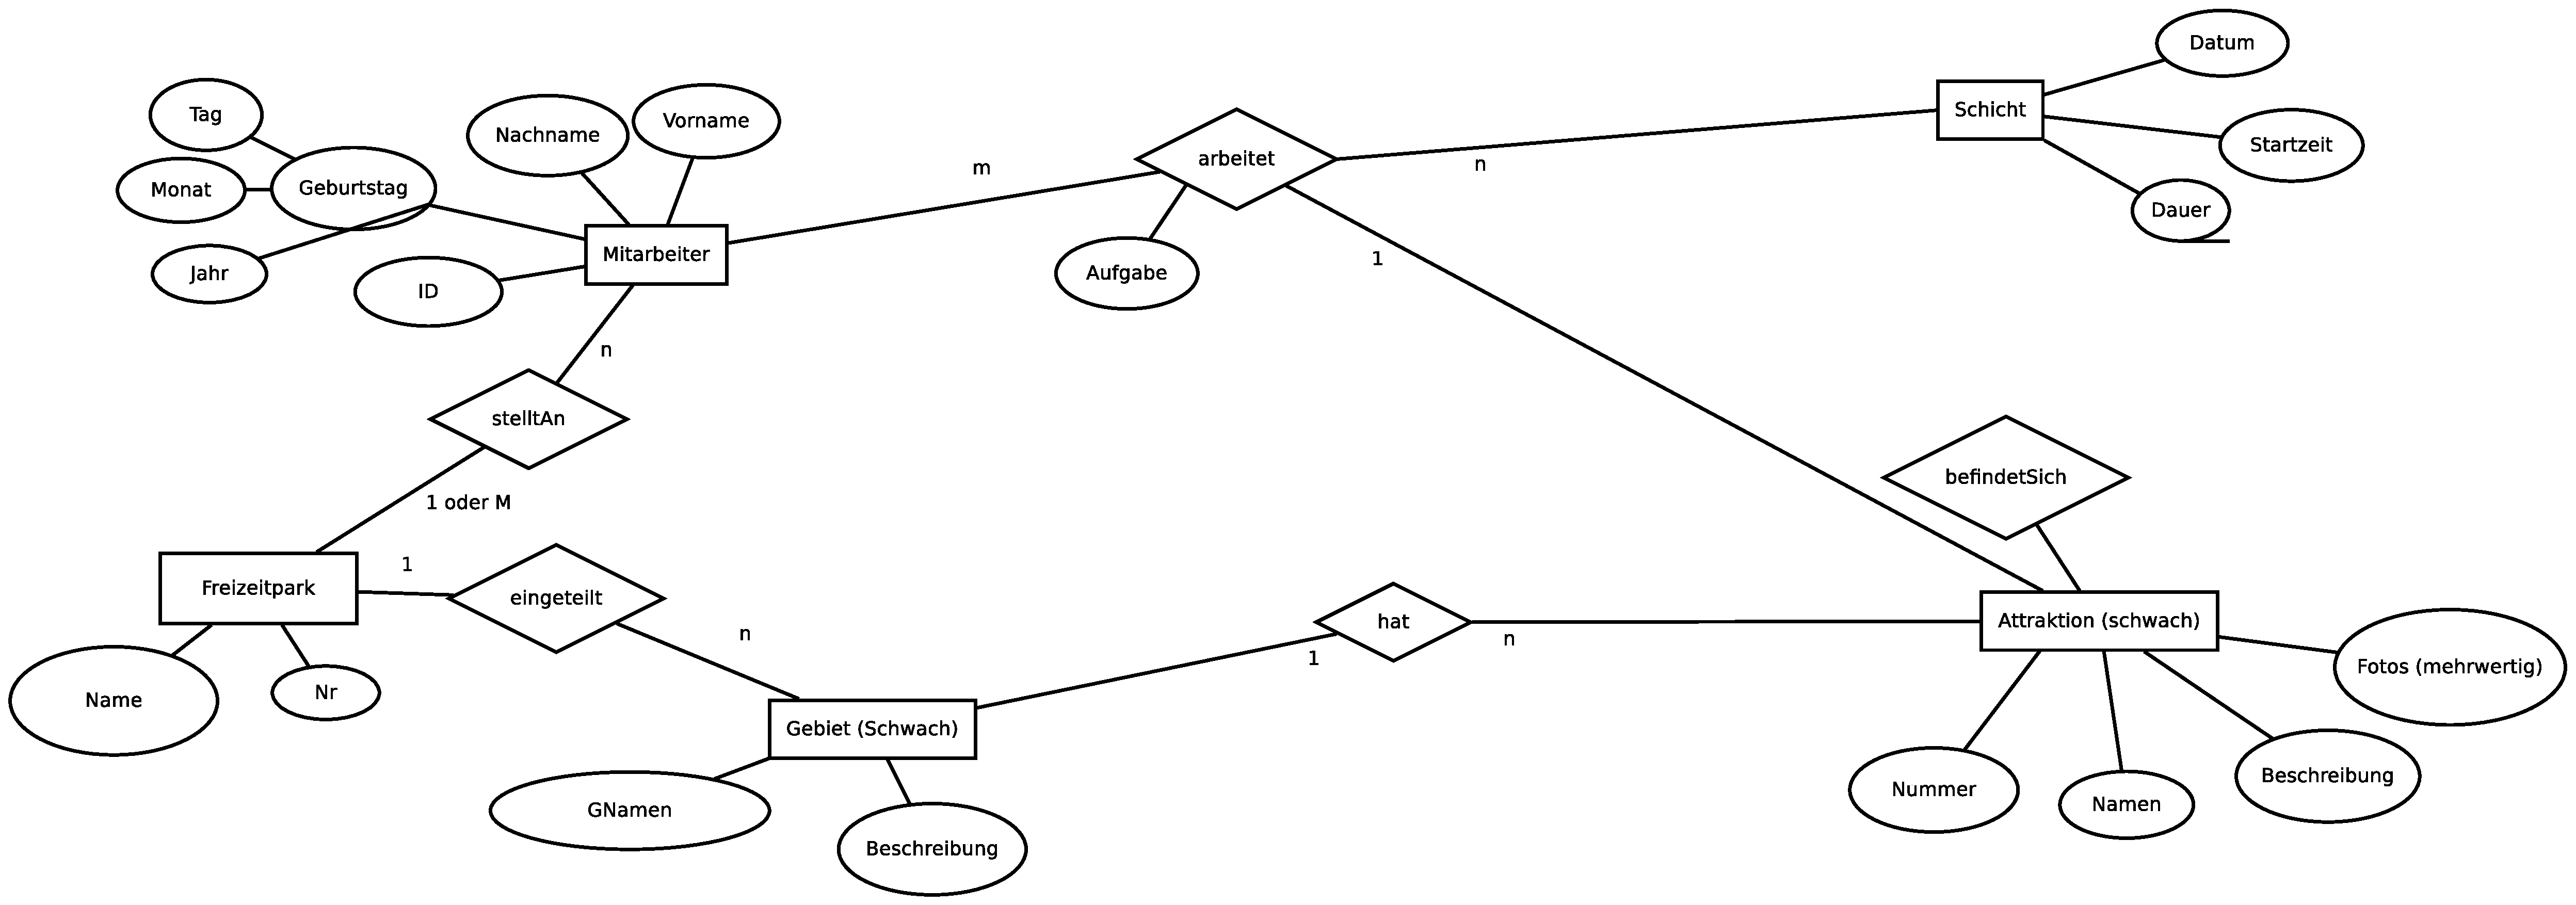
\includegraphics[width=\linewidth]{Freizeitpark.eps}

\begin{tikzpicture}[er2]
\node[entity] (Freizeitpark) {Freizeitpark};

\node[weak entity,right=4cm of Freizeitpark] (Gebiet) {Gebiet};

\node[entity,below=3cm of Freizeitpark] (Mitarbeiter) {Mitarbeiter};

\node[entity,below=3cm of Gebiet] (Schicht) {Schicht};

\node[weak entity,below right=3cm of Mitarbeiter] (Attraktion) {Attraktion};

\end{tikzpicture}
\end{document}
